\documentclass[11pt]{beamer}
\usetheme{CambridgeUS}

\usepackage[latin5]{inputenc}
\usepackage[T1]{fontenc}

\usepackage{graphicx}
\usepackage{media9}

\author{Alumna: Jenny Chavez \\ Profesor: Esp. Ing. Eric Pern�a (UNQ, FIUBA)}

\title{Protocolos de Comunicaci�n - Firmata}

\titlegraphic{
\includegraphics[width=3cm,height=0.9cm]{logo_FIUBA.jpg}
	   \hspace*{0cm}~%
	   
\includegraphics[width=4cm,height=1.5cm]{Proyectociaa.png}
 }
\subtitle{}

\setbeamercovered{transparent}
\setbeamertemplate{navigation symbols}{}
\setbeamertemplate{footline}[frame number]

\date{}

\begin{document}
	\maketitle
	\begin{frame}
		\frametitle{\centerline{Firmata}}
		\framesubtitle{Introducci�n}
		\begin{block}{
			Firmata es un protocolo para comunicarse con microcontroladores desde el software en una computadora (o tel�fono inteligente / tableta, etc.)}
		\end{block}
		\begin{itemize}
			\item {Protocolo abierto}
			\item {Simple}	
			\item {Basado en MIDI(Musical Instrument Digital Interface)}		
			\item {Comandos en Hexadecimal}
		\end{itemize}
	\end{frame}
	
	\begin{frame}
		\frametitle{\centerline{Firmata}}
		\framesubtitle{Implementaci�n}
		\begin{block}{
			 Este protocolo fue dise�ado para la comunicaci�n directa entre un microcontrolador y un objeto de software en una computadora host}
		\end{block}
		\begin{figure}[ht]
			\centering
			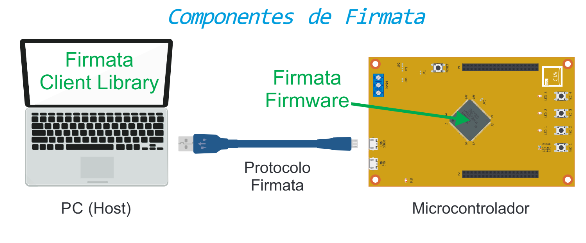
\includegraphics[width=0.8\textwidth]{ComponentesFirmata.png}
			\caption{Arquitectura de Firmata}
			\label{ig:anticitera}
		\end{figure}
	\end{frame}
	
	\begin{frame}
			\frametitle{\centerline{Firmata}}
			\framesubtitle{Tipos de mensaje}
			\begin{table}
				\begin{tabular}{c| c|p{1cm}| c|p{1cm} c|p{1cm}  p{1cm}}
					 \textbf{Tipo} & \textbf{Comando} & \textbf{Canal MIDI}& \textbf{Primer byte} & \textbf{Segundo byte}\\\hline
					analog I/O message& 0xE0& pin& LSB(bits 0-6)& MSB(bits 7-13)\\\hline
					digital I/O message& 0x90& port& LSB(bits 0-6)& MSB(bits 7-13)\\\hline
					report analog pin& 0xC0& pin& disable/enable(0/1)& - n/a -\\\hline
					report digital port& 0xD0& port& disable/enable(0/1)& - n/a -\\\hline
					start sysex& 0xF0& & \\\hline
					set pin mode(I/O)& 0xF4& & pin (0-127)& pin mode\\\hline
					set digital pin value& 0xF5& & pin (0-127)& pin value(0/1)\\\hline
					sysex end& 0xF7& & & \\\hline
				\end{tabular}
			\end{table}
	\end{frame}
	
	\begin{frame}
			\frametitle{\centerline{Firmata}}
			\framesubtitle{Ejemplos}
			\begin{block}{Comando 0xD0} 
			\end{block}
				\begin{block}
				 	{midi: transmite el mensaje de presi�n del canal MIDI}
				\end{block}
					\begin{block}
						{firmata: habilita la generaci�n de informes para un puerto digital (colecci�n de 8 pines)}
					\end{block}
			\begin{itemize}
				\item {PC: 0x91 0x01 0x00}	
			\end{itemize}
	\end{frame}
	
	\begin{frame}
		\frametitle{\centerline{Firmata4CIAA}}
		\framesubtitle{Implementaci�n}
		\begin{figure}
		\centering
		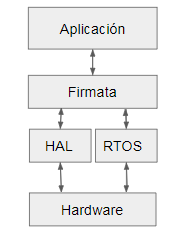
\includegraphics[width=0.4\textwidth]{capas.png}
	    \end{figure}
	\end{frame}
	
	\begin{frame}
		\frametitle{\centerline{Firmata4CIAA}}
		\framesubtitle{HAL}
		\begin{block}{Modulo}
			Maneja los perifiericos de una manera efectiva sin necesidad de usar los modulos propios del micro.
		\end{block}
			\begin{block}{Lo que se hizo:}
			\end{block}
			\begin{figure}
				\centering
				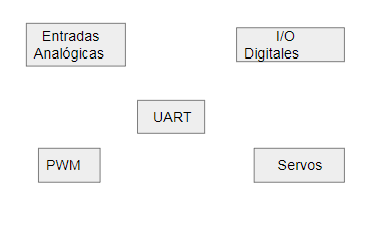
\includegraphics[width=0.5\textwidth]{hal.png}
				\caption{Primera parte}
				\label{fig:anticitera}
			\end{figure}
	\end{frame}
	
	\begin{frame}
		\frametitle{\centerline{Firmata4CIAA}}
			\framesubtitle{RTOS}
		\begin{block}{Maneja todas las tareas del sistema apropiativo:}
		\end{block}
		\begin{figure}
			\centering
			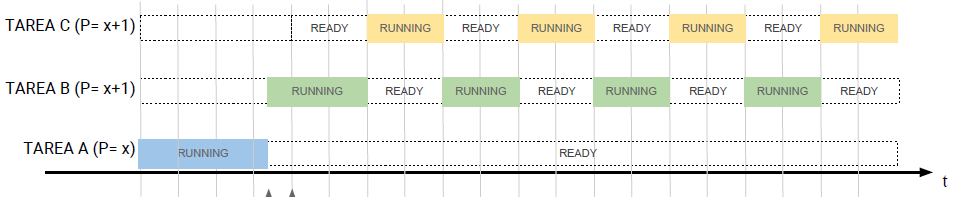
\includegraphics[width=0.7\textwidth]{tareas.png}
		\end{figure}
	\end{frame}
	
	\begin{frame}
			\frametitle{\centerline{Blockly}}
				\begin{block}{Es una biblioteca de JavaScript del lado del cliente para crear lenguajes de programaci�n de bloque visual y editores.}
				\end{block}
			\begin{figure}
				\centering
				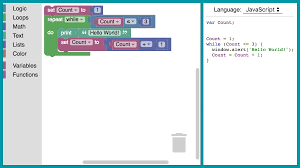
\includegraphics[width=0.5\textwidth]{blocky.png}
				\caption{The JavaScript Robotics Programming Framework}
				\label{fig:anticitera}
			\end{figure}
	\end{frame}	
	
		\begin{frame}
			\frametitle{\centerline{Blockly}}
			\begin{block}{
					Blockly es uno de un creciente n�mero de entornos de programaci�n visual.}
			\end{block}
			\begin{itemize}
				\item {	C�digo exportable}
				\item { Open source}	
				\item { Extensible}		
				\item {Altamente capaz}
			\end{itemize}
		\end{frame}


	\begin{frame}
	\frametitle{\centerline{Johnny five}}
	\framesubtitle{Cliente Firmata}
	\begin{figure}
		\centering
		
\includegraphics[width=0.5\textwidth]{johnny.png}
		\caption{The JavaScript Robotics Programming Framework}
		\label{fig:anticitera}
	\end{figure}
	\end{frame}	
	
	
		\begin{frame}
			\frametitle{\centerline{Johnny five}}
			\begin{block}{
					Johnny-Five es un marco de programaci�n de fuente abierta, basado en el protocolo Firmata, IoT y Rob�tica.}
			\end{block}
			\begin{itemize}
				\item {	nos facilitar� la comunicaci�n entre la aplicaci�n y la placa}
				\item { es JavaScript}	
			\end{itemize}
		\end{frame}			
	
	\begin{frame}
		\begin{center}
           {\fontsize{30}{40}\selectfont Integraci�n} 
		\end{center}
	\end{frame}
	
	\begin{frame}
		\begin{center}
			{\fontsize{20}{30}\selectfont Gracias!} 
		\end{center}
	\end{frame}
	
\end{document}

